\documentclass[10pt]{article}
\usepackage{icmlko}

\icmlmeta{IP 파운데이션 월드모델}{311}{선형이 더 잘 빌린다}{빌림이 나무에만 있을 것이라 예측하고 쟀다 --- 여섯 정식화가 다 같은 만큼 빌리고 문턱을 넘는 것은 선형쪽이다}

\begin{document}

\twocolumn[
\icmlheader

\begin{abstract}
노트 310이 ``달력 갈래의 다섯째 후보''를 남겼다 --- 달력은 도메인마다 다르게
작동하고(웹툰 · 애니에서 새롭고 세계애니 · 도서에서 아니다) \textbf{나무만
그 조건부를 표현하므로} 빌림이 나무 전용일 것이라는 가설이다. 선형은 달력
계수를 하나로 묶으니 옮길 것이 없다고 봤다. 쟀다. \textbf{틀렸다.} 정식화
여섯이 도서에서 \textbf{다 같은 만큼 빌린다} --- 나무 F18 0.1263 · F8 0.1123,
선형 F6 0.1143 · F9 0.1045 · F21 0.1111, 섞음 F23 0.1350. 몫으로도 31$\sim$37\%
로 붙어 있다. 그리고 \textbf{문턱을 넘는 것은 선형쪽이다} --- 도메인 문턱
$|t|{>}2.77$ 을 F6 3.52 · F9 3.45 · F21 3.30 · F23 3.14 가 넘고 나무 둘은
2.64 · 2.71 로 못 넘는다. 선형의 짝SE 가 더 작기 때문이다(0.030$\sim$0.034
대 0.042$\sim$0.048). \textbf{그러니 가설이 뒤집힌 정도가 아니라 반대다.}
생각해 보면 당연하다 --- \textbf{묶인 계수야말로 순수한 빌림}이다. 풀링
선형은 달력 계수 하나를 전 도메인에서 적합하고 그 계수는 웹툰 · 애니가
정한다. 도서 행은 남이 정한 계수를 그대로 받는다. 나무는 오히려 도메인
조건부를 만들 수 있어 \emph{덜} 빌릴 수도 있다. \textbf{덤으로 노트 303의
관측이 처음으로 문턱을 넘었다} --- 그때 F18 $t{=}{-}2.87$ 로 아슬아슬했던
것이 선형에서 3.5 다.
\end{abstract}
]

\section{가설은 나무 전용이었다}

노트 310의 마지막 절이 오래 열린 갈래(``달력이 왜 트리에서만 되는지'',
설명 넷 실패)에 다섯째 후보를 붙였다.

\begin{center}\small
\begin{tabular}{l}
\hline
달력은 도메인마다 다르게 작동한다 \\
\quad (웹툰 · 애니 ``새롭다'' · 세계애니 · 도서 아님) \\
나무만 그 조건부를 표현한다 \\
\hline
$\Rightarrow$ \textbf{빌림도 나무에만 있어야 한다} \\
\hline
\end{tabular}
\end{center}

논리가 깔끔해 보였다. 선형은 달력 계수를 하나로 묶으니 ``웹툰에서 배운 달력
구조를 도서 행에 옮긴다''는 말이 성립할 자리가 없어 보였다.

\paragraph{방법} 노트 303 · 310과 같다 --- 도서의 ``안 오른다'' 축 아홉을
도서에서만 끄고(값 0.5 · 표시자 0) 유보 $\rho$ 가 얼마나 내려가는지 본다.
정식화만 갈아 끼운다.

\section{여섯이 다 같은 만큼 빌린다}

\begin{figure*}[t]
\centering
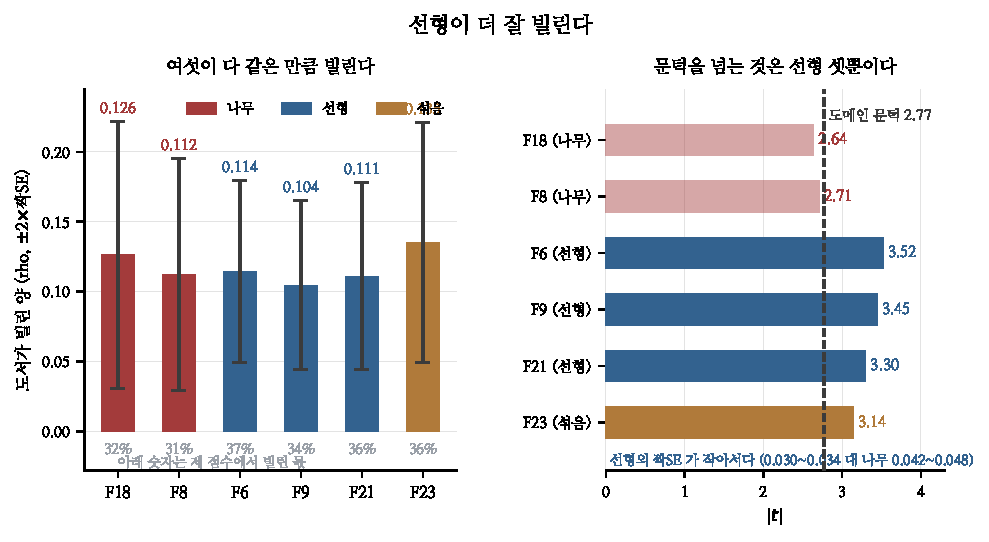
\includegraphics[width=\textwidth]{figs/pooled.pdf}
\caption{왼쪽 --- 정식화별로 도서가 빌린 양($\pm$2$\times$짝SE, 부트스트랩
400). 오른쪽 --- 같은 것의 $|t|$ 와 도메인 문턱.}
\end{figure*}

\begin{center}\footnotesize
\begin{tabular}{llrrrrr}
\hline
정식화 & 무리 & 원래 & 막음 & 빌림 & $t$ & 몫 \\
\hline
F18 & 나무 & 0.3895 & 0.2632 & 0.1263 & $-$2.64 & 32\% \\
F8 & 나무 & 0.3675 & 0.2552 & 0.1123 & $-$2.71 & 31\% \\
\textbf{F6} & \textbf{선형} & 0.3108 & 0.1965 & 0.1143 & \textbf{$-$3.52} & 37\% \\
\textbf{F9} & \textbf{선형} & 0.3055 & 0.2010 & 0.1045 & \textbf{$-$3.45} & 34\% \\
\textbf{F21} & \textbf{선형} & 0.3118 & 0.2007 & 0.1111 & \textbf{$-$3.30} & 36\% \\
F23 & 섞음 & 0.3754 & 0.2404 & 0.1350 & \textbf{$-$3.14} & 36\% \\
\hline
\end{tabular}
\end{center}

\textbf{빌린 양이 0.1045$\sim$0.1350 으로 붙어 있다.} 몫도 31$\sim$37\%다.
무리로 갈리지 않는다.

\paragraph{그리고 문턱을 넘는 것은 선형쪽이다} 도메인 문턱
$|t|{>}2.77$(노트 275 · 282)을 F6 · F9 · F21 · F23 이 넘고 \textbf{나무 둘은
못 넘는다.} 값이 비슷한데 $t$ 가 갈리는 이유는 짝SE 다.

\begin{center}\small
\begin{tabular}{lrr}
\hline
무리 & 빌림 & 짝SE \\
\hline
나무 & 0.1123 $\sim$ 0.1263 & 0.042 $\sim$ 0.048 \\
\textbf{선형} & 0.1045 $\sim$ 0.1143 & \textbf{0.030 $\sim$ 0.034} \\
\hline
\end{tabular}
\end{center}

노트 296이 잰 것과 같은 무늬다 --- 나무는 같은 자료 변화에 \textbf{크고
방향 없는} 반응을, 선형은 \textbf{작고 한 방향인} 반응을 낸다. 그때는 팝업
16행에서 여덟 배였고, 여기서는 도서 163행에서 한 배 반이다.

\section{생각해 보면 반대여야 했다}

\begin{center}\small
\begin{tabular}{ll}
\hline
내가 생각한 것 & 빌림 ${=}$ 도메인 조건부 구조를 옮기는 것 \\
& $\Rightarrow$ 나무만 가능 \\
\hline
\textbf{실제} & 빌림 ${=}$ \textbf{남이 정한 계수를 받는 것} \\
& $\Rightarrow$ \textbf{묶인 계수가 제일 순수하다} \\
\hline
\end{tabular}
\end{center}

풀링 선형(F6)은 달력 계수 \emph{하나}를 전 도메인에서 적합한다. 그 계수는
행 수로 웹툰 2,106 · 애니 1,467 이 정하고 도서 80 은 거의 못 정한다.
\textbf{도서 행은 남이 정한 계수를 그대로 받는다} --- 그것이 빌림의 정의
그대로다.

나무는 오히려 도메인 조건부를 만들 \emph{수} 있으므로 \textbf{덜} 빌릴
여지가 있다. 실제로 나무 둘의 빌린 몫(31 · 32\%)이 선형 셋(34 · 36 · 37\%)보다
조금 낮다 --- 다만 그 차이는 짝SE 안이다.

\paragraph{그래서 달력 갈래의 다섯째 후보는 죽는다} 달력이 나무에서만 되는
이유가 ``나무만 빌릴 수 있어서''는 아니다. 선형도 빌리고 오히려 더 안정적으로
빌린다. \textbf{설명 다섯째도 실패다} --- 관측으로 둔다.

\section{덤 --- 노트 303의 관측이 문턱을 넘었다}

노트 303이 도서 빌림을 $t{=}{-}2.87$ 로 냈고 도메인 문턱 2.77 을 겨우
넘었다(위키 정정 뒤 다시 재니 $-$2.54 로 못 넘었다). \textbf{선형에서는
3.30$\sim$3.52 다.}

\begin{center}\footnotesize
\begin{tabular}{lrl}
\hline
노트 & $t$ & \\
\hline
303 (F18, 정정 전) & $-$2.87 & 겨우 넘음 \\
309 대조 (F18, 정정 후) & $-$2.54 & 못 넘음 \\
\textbf{311 (F6)} & \textbf{$-$3.52} & \textbf{넘음} \\
\hline
\end{tabular}
\end{center}

\textbf{빌림이라는 현상 자체가 처음으로 확실해졌다.} 정식화를 갈아 끼우는
것이 표본을 늘리는 것과 같은 일을 했다 --- 잡음이 작은 자로 다시 잰 것이다.

\paragraph{남은 것}
\begin{center}\small
\begin{tabular}{ll}
\hline
갈래 & 왜 \\
\hline
빌림은 선형으로 재라 & 짝SE 가 3분의 2다 \\
펀딩도 여섯 정식화로 & 도서와 같은 무늬인가 \\
달력 갈래 & 설명 다섯째도 실패 --- 관측으로 \\
피처 위약의 꼬리 & 다섯 건이 답을 정한다 \\
\hline
\end{tabular}
\end{center}

\paragraph{규약} \textbf{현상을 재는 자를 고를 때 잡음이 작은 자를 쓰라 ---
그 자가 챔피언이 아니어도.} 이 실험실은 판 $\rho$ 로 F18 을 챔피언으로
뽑았고 그래서 모든 것을 F18 로 쟀다. 그런데 \emph{빌림}이라는 현상은 F6 이
훨씬 또렷하게 보여 준다(짝SE 0.032 대 0.048). \textbf{순위를 정하는 자와
현상을 재는 자는 같을 이유가 없다.} 그리고 \textbf{깔끔한 논리를 재 보라}
--- ``선형은 조건부를 못 하니 못 빌린다''가 너무 그럴듯해서 안 쟀으면
반대 방향을 못 봤을 것이다.

\end{document}
